\section{Method}\label{sec:Method}


\subsection{Simple Terrain Approximation}

Instead of jumping straight to real world terrain data, we'll explore how
polynomial regression works on synthetic terrain. The \textit{Franke function}
has features similar to those one would expect from terrain with smooth hills
and valleys. For simplicity we'll only to model the domain \(x, y \in [0,
1]\), for which the Franke function is plotted in~\cref{fig:franke}.


\begin{figure}[]
  \centering
  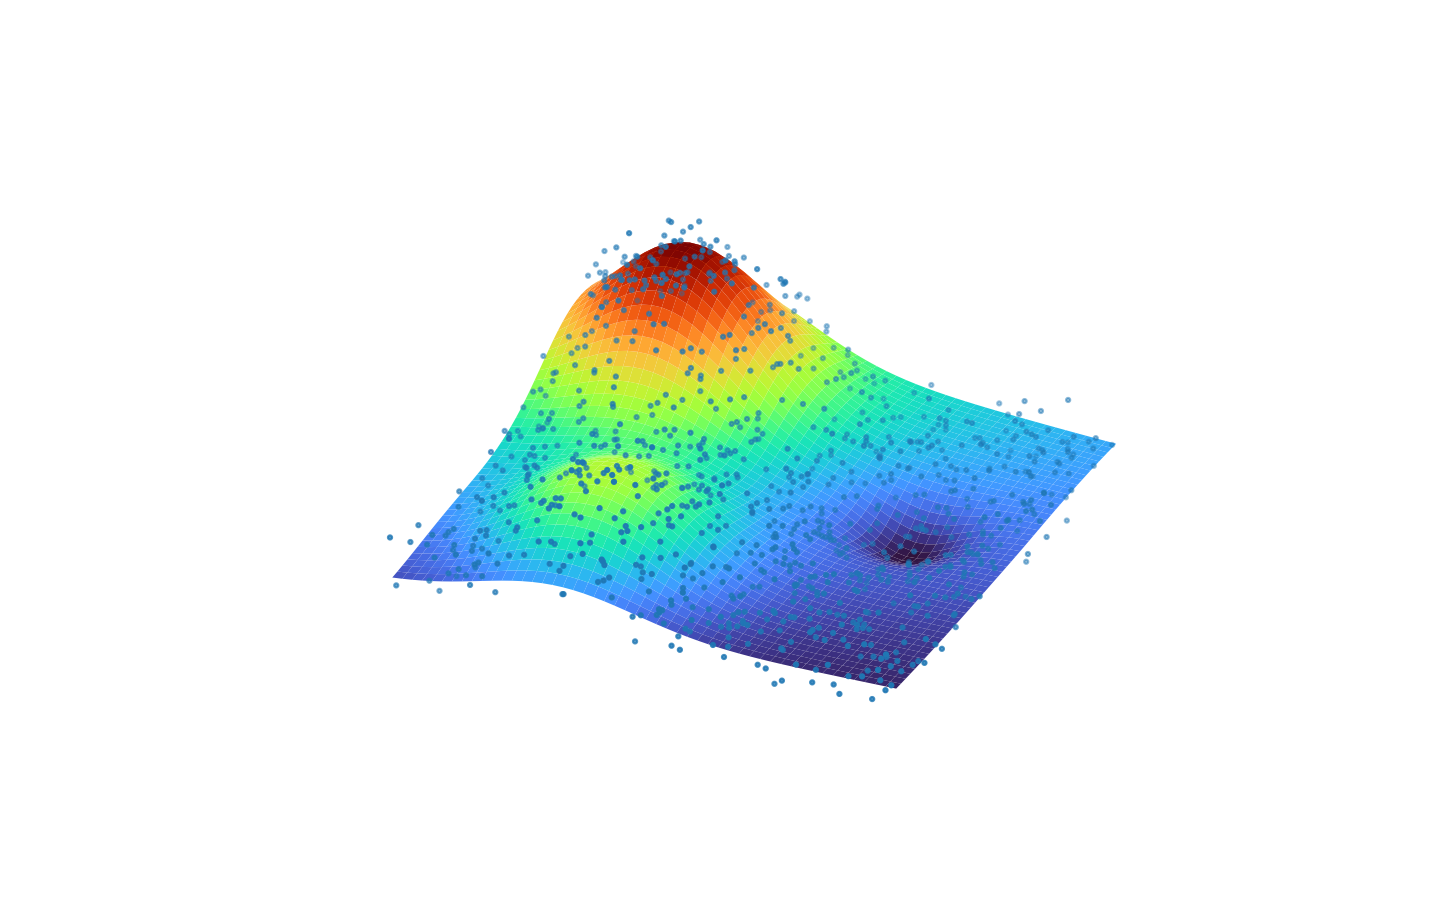
\includegraphics[trim={2cm 1cm 1cm 1cm},clip]{figures/franke.png}
  \caption{\label{fig:franke} Visualization of the Franke function in the domain
   \(0 \leq x, y \leq 1\) colored by height. A random sample of 100 points are
   also shown.}
\end{figure}

\subsection{Real World Terrain Data}
\label{sec:real-world-terrain}

The real world terrain data was retrieved from
\href{https://earthexplorer.usgs.gov/}{Earth Explorer} over the Vestfold area.

I found it unrealistic for the polynomial model to be able to fit the terrain to
any reasonable degree, so I decided to down-sample the terrain by a factor of
\(50\). The original and down-sampled terrain are shown in~\cref{fig:terrain}

\begin{figure}[]
  \centering
  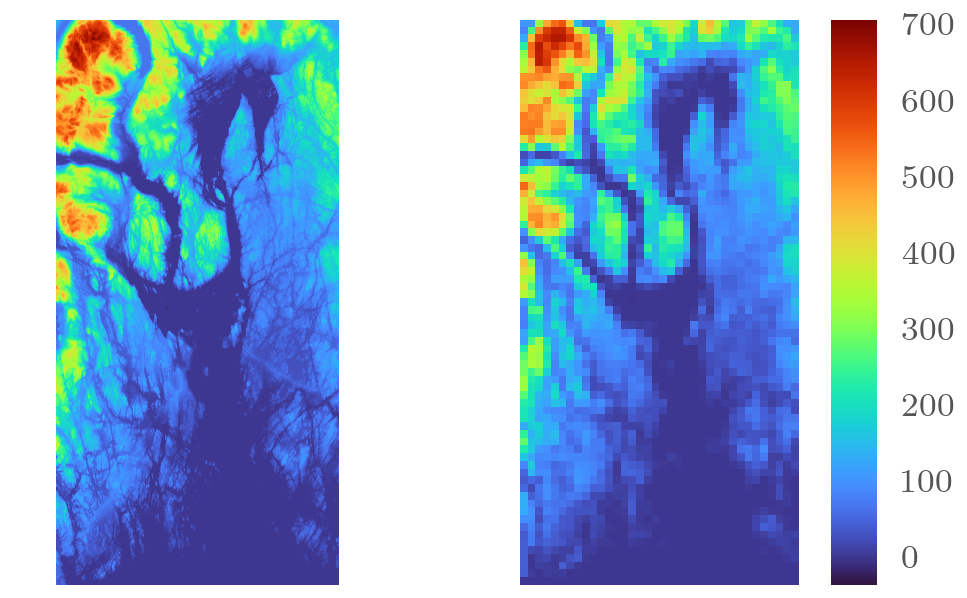
\includegraphics[]{figures/terrain.png}
  \caption{\label{fig:terrain} Digital terrain data over Vestfold. The plot on
    the right is down-sampled by a factor \(50\). The terrain is colored by
    height using the
    \href{https://ai.googleblog.com/2019/08/turbo-improved-rainbow-colormap-for.html}{turbo
    colormap}.}
\end{figure}


\subsection{Implementation Details}

When fitting a model, a sample of \(100\) observations is drawn from the domains
of \(x\) and \(y\)
\(\text{franke}(\vb{x}, \vb{y})\) is computed. Gaussian noise \(\vb{\varepsilon}
\sim \mathcal{N}(0, 0.1)\) is added. The terrain is mapped to \((0, 1)\) to
prevent large numbers in the construction of the design matrix. This is all done in the \texttt{Sampler}
class.


To examine the behavior of the different regression methods, many models must be
fitted to the data and their results recorded. This book-keeping is hid under the rug using the
\texttt{Runner} class, allowing us to easily study the effects of
hyperparameters and model complexity.


Monte Carlo simulations are used for decomposing the MSE into squared bias and
variance by regressing on perturbated \(y_{i}\). This is done in the
\texttt{Ensemble} class.


All of the results presented in this paper can be perfectly reduplicated by running the
corresponding cells in the Jupyter Notebook as the random seed is set at each
call to \texttt{Sampler}.

All of the core code is tested against equivalent methods in the sklearn
library, while much of the ``bookkeeping'' code is untested to save time. The
tests themselves are tested using mutation testing with the Cosmic Ray package.